%%%
%%% Chapter
%%%
\chapter{Data Analysis}
\label{chap:DataAnalysis}


%%%%%%%%%%%%%%%%%%%%%%%%%%%%%%%%%%%%%%%%%%%%%%%%%%%%%%%%%%%%%%%%%
\section{Estimation}
\label{sec:Estimation}


%%%%%%%%%%%%%%%%%%%%%%%%%%%%%%%%%%%%%%%%%
%%%%%%%%%%%%%%%%%%%%%%%%%%%%%%%%%%%%%%%%%%%%%%%%%%%%%%%%%%%%%%%%%%%%%%
\section{Simple Monte Carlo Evaluation of Integrals}
It is the purpose of this subsection to introduce Monte Carlo Methods
in the context of the numerical evaluation of definite integrals.
We will see in later chapters that Monte Carlo integration is the
method of choice when treating multidimensional
integrals numerically. As a typical rule of thumb
``classical'' deterministic methods are outperformed
by Monte Carlo methods  for systems with a large number of 
degrees of freedom.
For simplicity and to stress the basic ideas 
it is convenient at the moment to consider one--dimensional definite
integrals of the form
\begin{equation}
\label{INTEGRAL}
I = \int_a^b dx f(x).
\end{equation}
Obviously such integrals can be evaluated analytically for many
integrands
$f(x)$.  However, there are as well many cases for which a numerical
evaluation is necessary.

Before introducing the Monte Carlo approach to numerical integration
let us remind the basic ``classical'' deterministic approach to
numerical integration. The standard approach is based upon the
geometrical interpretation of the integral (\ref{INTEGRAL}) as the
area under the curve of the function $f(x)$ between the points $a$ and
$b$. In the simplest algorithm this area (see figure) is approximated
as a sum over rectangles. To this end the $x$--axis is divided into
$n$ equally spaced intervals of width $\Delta x$,
\begin{equation}
\Delta x = \frac{b-a}{n}
\end{equation}
whose ends are given by
\begin{equation}
x_i = x_0 + i\Delta x
\end{equation}
for $i=1, \ldots ,n$. Of course, $x_0 = a$ and $x_n =b$. Thus in the
so--called rectangular approximation the integral is evaluated as
\begin{equation}
\label{I_CLASSICAL}
I_n = \Delta x \sum_{i=0}^{n-1} f(x_i).
\end{equation}
Of course, other more accurate approximations are possible.

How can we now evaluate the above integral by drawing random numbers?
The standard way is based on a very simple idea. 
From the introductory course in analysis we know that the Mean 
Value Theorem states that the exact value of the integral $I$ is 
given by
\begin{equation}
I= (b-a) f(\zeta)
\end{equation}
for some value of $\zeta$ in the interval $a \le \zeta \le b$. $f(\zeta)$
represents the average value of the function $f(x)$ 
in the interval $[a,b]$. Thus we could also write
\begin{equation}
I = (b-a) \langle f \rangle,
\end{equation}
where $\langle  \rangle$ denotes the mean value.
Let us draw $n$
random numbers which are uniformly distributed in the interval $[a,b]$
and let us sample the corresponding value of $f(x_i)=f_i$. The Monte Carlo
estimate $I_n$ of the integral $I$ is then the sample mean, which is
given by
\begin{equation}
\label{MCI_STANDARD}
I_n = \frac{(b-a)}{n} \sum_{i=1}^{n} f(x_i),
\end{equation}
where $n$ is the number of trials. Amazingly the form of the above
estimate is very similar to the classical formula (\ref{I_CLASSICAL}).
The fundamental difference is that now the $n$ points at which the
function $f$ is evaluated are no longer equally spaced but randomly 
distributed.

There is also the possibility to compute the integral $I$
stochastically
with the help of the ``Hit or Miss'' algorithm. The idea behind
this algorithm is again very simple. To be explicit we imagine a rectangle
of height $h$ and width $(b-a)$ such that the function $f(x)$ lies
within the rectangle (see figure; Gould, p.329). To evaluate the
integral we draw randomly pairs of uniformly distributed random
numbers $(x_i,y_i)$ such that $a \le x_i \le b$ and $0 \le y_i \le h$.
In other words the probability to draw a point within the rectangle is
given by the inverse of the area $A$ of the rectangle,
i.e. $1/(b-a)h$. It is now evident how the area under the
function $f$ may be estimated. The fraction of points $(x_i,y_i)$
which satisfy the condition $y_i \le f(x_i)$ is an estimate of the
ratio of the integral $I$ to the area $A$ of the rectangle. Hence,
drawing $n$ random pairs the estimate $I_n$ of $I$ by this ``scoring''
method is given by
\begin{equation}
I_n = A \frac{n_s}{n},
\end{equation}
where $n_s$ is the number of ``hits'', i.e., of points lying below the
curve $f(x)$.

Before writing two simple programs to elucidate the above algorithms
it is important to have in mind that both estimates are affected by
statistical errors. Let us consider for simplicity 
the standard method. Since the $f(x_i)$ are random we know 
from the elementary theory of data analysis
that an appropriate measure of the error is given by the variance
which is defined by
\begin{equation}
{\rm Var}(f) = \langle f^2 \rangle - \langle f \rangle^2.
= \langle (f -\langle f \rangle)^2 \rangle
\end{equation}
Since we draw a finite number of random numbers we can
estimate the mean value by using
\begin{equation}
\hat{f}  = \frac{1}{n} \sum_{i=1}^n f(x_i) 
\end{equation}
and correspondingly the estimate of the variance by using
\begin{equation}
{\rm Var}(f(x_1),\ldots, f(x_n)) = \frac{1}{n-1} \sum_{i=1}^n 
   (f(x_i)- \hat{f})^2 = \sigma_f^2.
\end{equation}
The quantity $\sigma_f = \sqrt{{\rm Var}(f_1, \ldots, f_n)}$ 
is also called the standard deviation. In the previous expression
we have used the short--hand
notation $f(x_i) = f_i$. However,
we are not interested in the error of $f$ but in the error of the
estimate $I_n$, which is a sum over random numbers. 

Repeating the 
simulation and hence drawing other random numbers we will get another
estimate of $I_n$. Therefore, repeating the simulation $m$ times 
we can estimate the mean of $I_n$ as
\begin{equation}
\hat{I_n} = \frac{1}{m} \sum_j^m I_n(j)
\end{equation}
and the corresponding variance as
\begin{equation}
{\rm Var}(I_n(1), \ldots, I_n(m)) = 
\frac{1}{m-1} \sum_j^m (I_n(j) - \hat{I_n})^2 = \sigma_I^2
\end{equation}
We will denote the above variance also by $\sigma_I^2$.
Of course, proceeding this way is not very practical since we
have to perform the simulation $m$ times. A much more economical
estimation of the error of the mean of $I_n$ could be achieved by 
establishing a simple relation between $\sigma_I$ and the standard 
deviation of the individual trials $\sigma_f$. To this end we 
introduce the discrepancy $\delta f_i$ between the
individual trial $f_i$ and its mean $\langle f \rangle$. The 
discrepancy $\delta I_n$ between $I_n$ and its mean value can be
obtained to first order in the $\delta f_i$ by a simple Taylor 
expansion (error propagation rules)
\begin{equation}
\delta I_n = \sum_{i=1}^n \frac{\partial I_n}{\partial f_i} \delta 
f_i.
\end{equation}
Hence, it follows from the above equation by taking the average over
$\delta I_n^2$ that
\begin{equation}
\langle \delta I_n^2 \rangle = \sum_{i,j=1}^{n}
    \frac{\partial^2 I_n}{\partial f_i \partial f_j} 
     \langle \delta f_i \delta f_j \rangle.
\end{equation}
It is plausible to assume, that 
$\langle \delta f_i \rangle = 0$
for all $i$ and that the $\delta f_i$ are not correlated
for $i \neq j$, i.e.,
$\langle \delta f_i \delta f_j \rangle = \langle f_i \rangle \langle f_j \rangle$
and that for $i=j$ we have $\langle \delta f_i^2 \rangle = \sigma_f$ 
for all $i$ it follows from the above equation that
\begin{equation}
\sigma_I^2 = \sum_{i=1}^n \left(
      \frac{\partial I_n}{\partial f_i} \right)^2 \sigma_f^2
      = \frac{1}{n^2} n \sigma_f^2 = \frac{\sigma_f^2}{n}
\end{equation}
and finally we have the useful relation
\begin{equation}
\sigma_I = \frac{\sigma_f}{\sqrt{n}}.
\end{equation}
The mean error of the mean scale with 1 over the square root of 
the number of individual trials. The precision of the estimate 
thus increases only slowly with the number of trials (remark: central
limit theorem: see Chapter 2).

Now we are in the position to write two programs to implement the above
stochastic algorithms. In order to be specific we compute the integral
\begin{equation}
I = \int_0^1 dx \sqrt{1-x^2} = \frac{\pi}{4}.
\end{equation}
In other words we want to estimate the number $\pi$ by Monte Carlo
methods.

We begin by the standard method. The listing of an according 
program can be seen below.

\subsubsection{Listing of the program mcpi.}
\inputlisting{./Listings/mcpi.m}

We run the program for $n=10, 100, 1000, 10000$. The result of the 
four simulations can be seen in Fig. xy.
\begin{figure}
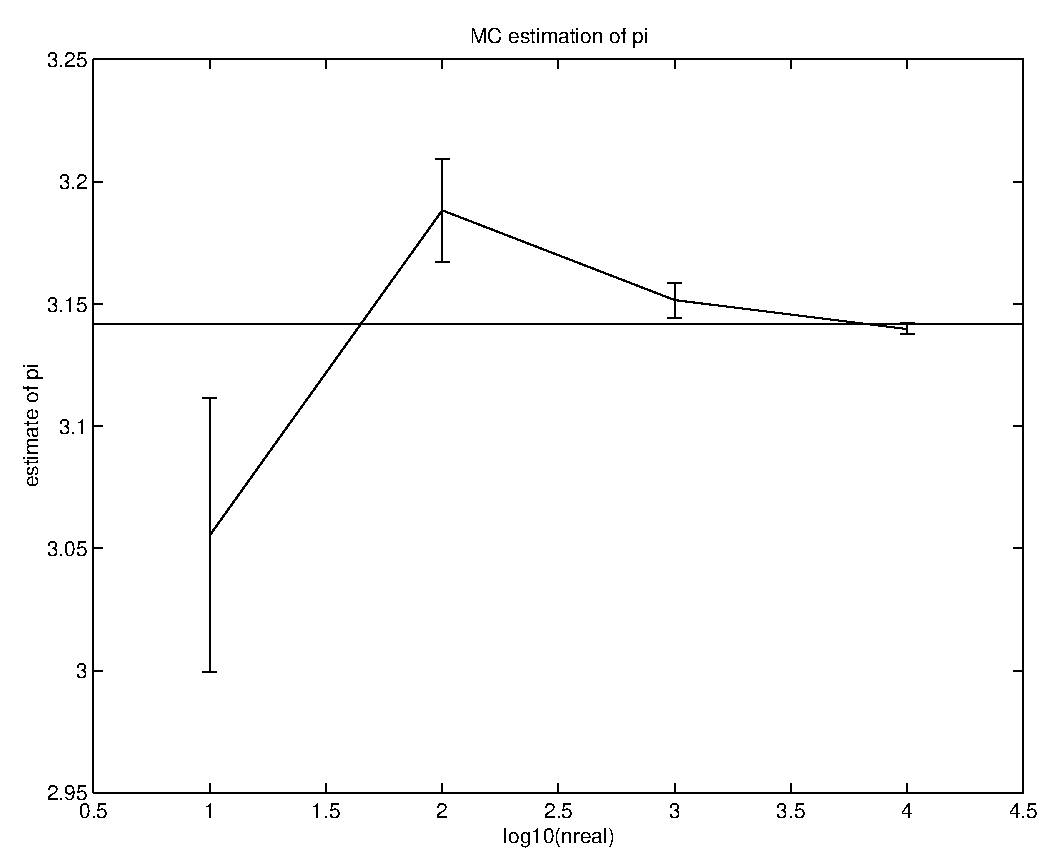
\includegraphics[width=\textwidth]{Figures/plotmcpi.eps}
\caption{The estimation of pi for n=10,100,1000,10000. The 
error bars correspond to the standard deviation of the mean of the 
estimate.}
\end{figure}

Next we write a program for the scoring  method. 

\subsubsection{Listing of the program mcpiscore.m}
\inputlisting{./Listings/mcpiscore.m}

Again we run the simulation for n=10, 100, 1000, 10000.
The result of a simulation can be seen in the next Figure.
\begin{figure}
\begin{center}
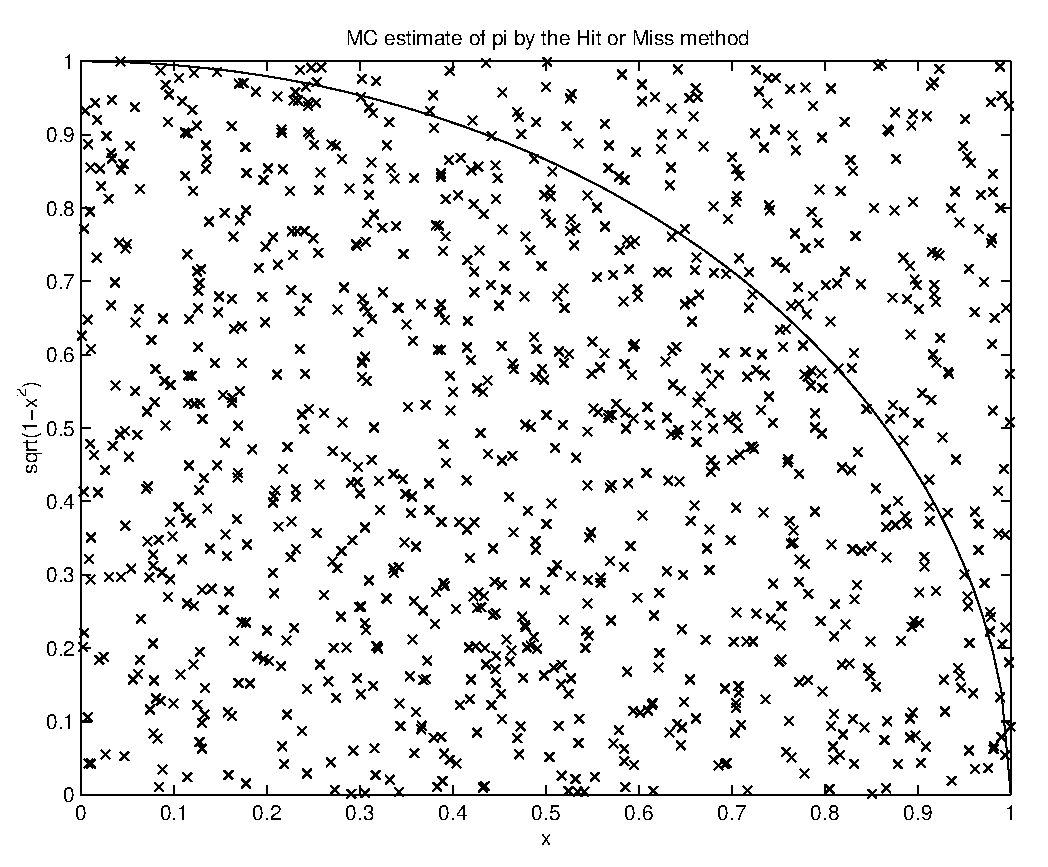
\includegraphics[width=.7\textwidth]{Figures/fmcpiscore.eps}
\end{center}
\caption{The scoring method. The continuous line represents
the function $\sqrt{(1-x^2)}$.}
\end{figure}


%%%%%%%%%%%%%%%%%%%%%%%%%%%%%%%%%%%%%%%%%%%%%%%%%%%%%%%%%%%%%%%%
\section{Beyond this chapter}


%%%%%%%%%%%%%%%%%%%%%%%%%%%%%%%%%%%%%%%%%%%%%%%%%%%%%%%%%%%%%%%%
\section{Exercises}

Use the  Matlab function \texttt{rand()}
to solve the following problems (don��t care about the quality and
the algorithm of the random number generator, for now):

\begin{Ex}
\label{Photoabsorption}
\textbf{Photoabsorption \cite[]{reif:67}} \\
Consider the absorption of photons passing through a gas in two dimensions.
We model the gas by introducing slabs of width $dx$ and density $n$ (in
particles per area), which absorb the incident photons. The slab
particles have a cross-sectional area of $\sigma$.

So the probability of a photon to be absorbed in the slab will be
($M$ is the number of particles in the slab of the height $dy$)
$$ P(\text{Photon absorbed}) = \frac{M\sigma}{dy} =
      \frac{\sigma n dx dy}{dy} = \sigma n dx  \quad .$$
We have assumed that there is no overlap between the cross-sections of
the slab particles.

Write a program to simulate this process on the computer. Take $N$
incident photons and watch the number of particles left over
against the slabs passed in a diagram. Do this simulation several
times and calculate the ensemble-average. What process you know
is similar to this behaviour and what takes the place of the spatial
dimension in that case?

%If we now have N identical slabs in a row, the probability of passing
%through all the slabs would be $(1-p)^N$, if the transmissions
%are statistically independent of each other.
%Then for a slab of finite thickness $X=N dx$ with $N\to\infty$, we
%get the Transmission probability
%$$ P(\text{transmitted through $N$ slabs}) =
%       \left(1-\frac{n\sigmaX}{N}\right)^N \quad .$$

%Now simulate the following systems:
%identical photons are absorbed in one slab ($N$ slabs)
\end{Ex}

\begin{Ex}
\label{Monte-Carlo_Integration}
\textbf{Monte-Carlo Integration -- Speed and Accuracy} \\
Write a program for the calculation of the following integral:
$$ \int_0^1 \frac{1}{1+x^2} dx\quad .$$
\begin{enumerate}
\item using the hit and miss method
\item using the standard method
\end{enumerate}
For both algorithms, calculate the mean and the standard deviation
as discussed in the lecture. Also use the analytical result of the
integral to calculate $\pi$. Compare the accuracy of both algorithms
using the approximations of $\pi$. Compare the speed of the two
programs by using the \texttt{cputime} function in Matlab.
(e.g. type the following to time the random number generator:
\texttt{t=cputime;x=rand(1000);cputime-t})

To that end, create a table and a plot with the two parameters
($n$: the number of intervals and $N$: the number of realizations)
against
the accuracy (use at least 5 values). To save time, you can first
check for a good $n$  and then do the plots only against $N$.
For the speed, plot the cputime against the achieved accuracy for
many different $N$.
\end{Ex}

\begin{Ex}
\label{Euler_Constant}
\textbf{Euler��s Constant using Monte-Carlo Algorithm %
          \cite[]{mohazzabi:98}} \\
Suppose throwing $N$ darts randomly at a dart board, which has been
divided into $R$ equal size regions. The probability of hitting one region
is $p=1/R$. Then the probability of hitting an empty region
(not already occupied by a dart) is $(1-p)^N$. Using the binomial
distribution, you can get the probability for hitting a region with
$m$ darts. If you choose
the number of regions equal to the number of darts
thrown on the board, we have $p=1/N$ and therefore
$$ P(\text{hitting an empty region}) = \left( 1-\frac{1}{N} \right)^N\quad .$$

Because the above series converges to $e$ for $N\to\infty$, we can use
the following method to get an approximation of the Euler constant:
\begin{enumerate}
\item[(i)] Throw randomly a large number of darts (say $N$) on a board, which has
  been divided into $N$ equal size regions.
\item[(ii)] Count the number of empty regions (call it $N_0$).
\item[(iii)] The fraction $N/N_0$ is a good estimate of the Euler constant $e$.
\end{enumerate}

Write a program for that algorithm and check the results. You can even
use $N/N_1$, if $N_1$ is the number of regions with the occupancy of
one dart. Check this, too. What $N$ do you need to
get the same accuracy using the formula? And how many terms of the
series for $e$ ($\sum_{i=0}^\infty 1/i! = e$)?
\end{Ex}

%%%%%%%%%%%%%%%%%%%%%%%%%%%%%%%

\bibliographystyle{Bibliographies\SimulationBook}
\bibliography{Bibliographies\V_98,Bibliographies\simulit}
